\documentclass{standalone}
\usepackage{tikz}
\usepackage{pgfplots}
\pgfplotsset{compat=1.18}
\pgfplotsset{ticks=none,axis x line=bottom,axis y line=left,enlargelimits=false}

\begin{document}
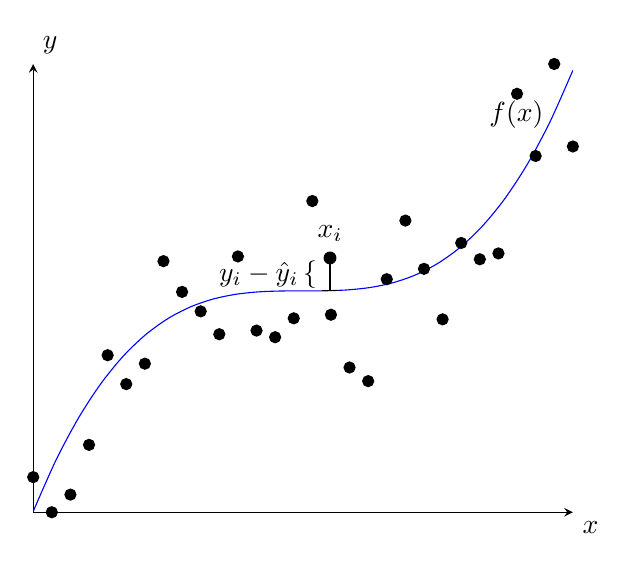
\begin{tikzpicture}
\begin{axis}[
    xlabel=$x$,ylabel=$y$,
    xlabel style={at={(ticklabel* cs:1)},anchor=north west},
    ylabel style={at={(ticklabel* cs:1)},anchor=south west},
    ylabel style={rotate=-90},]
    \addplot[only marks,samples=30]{0.75*x^3+40*rand};
    \addplot[blue, smooth]{0.75*x^3} node[pos=0.90](fx){};
    \draw(fx)node[left]{$f(x)$};
    \draw (0.5,14)node[draw, fill=black, circle, inner sep=1.5pt, label={$x_i$}]{};
    \draw[-|](0.5,14)--(0.5,0.09375)node[midway, left]{$y_i-\hat{y}_i\left\{\right.$};
\end{axis}
\end{tikzpicture}
\end{document}